\documentclass[12pt]{report}

\usepackage{geometry}
\geometry{ b4paper, total={220mm,320mm}, left=20mm,
            top=15mm, headheight=33pt,includeheadfoot}

\usepackage{mathtools}
\usepackage{bm}
\usepackage{graphicx}
\usepackage{listings}
\usepackage{tikz}
\usepackage{fancyhdr}
\pagestyle{fancy}

\usepackage{caption, subcaption, zref-totpages}

%\usepackage{libertine, lato}

\usepackage{amssymb}
\usepackage{enumitem}
\usepackage{amsmath}


\usepackage{fontspec}

%\usepackage{microtype}

\usepackage{polyglossia}

\usepackage{hyperref}
\hypersetup{
    colorlinks=true,
    linkcolor=blue,
    filecolor=magenta,      
    urlcolor=cyan
}
\urlstyle{same}

\rhead{
\includegraphics[width=1cm]{ece.png}}
\lhead{
\includegraphics[height=1cm]{uowm.png}}

\fancyfoot{}
\fancyfoot[RO]{\thepage /\ztotpages}

\graphicspath{ {img} }

\setmainfont[Numbers=Lining]{Georgia}
\setsansfont{Lato}
\setmonofont{Corbel}

\usetikzlibrary{arrows.meta}

\renewcommand{\thesection}{\Roman{section}}
\renewcommand{\thesubsection}{\thesection.\Roman{subsection}}

\title{\textsf{Εργαστηριο 2: Διαμόρφωση Πλάτους (ΑΜ)\\
    \large Τμήμα Ηλεκτρολόγων Μηχανικών \& Μηχανικών Υπολογιστών \\
    Πανεπιστήμιο Δυτικής Μακεδονίας
}}
\author{\textsf{Μάρκος Δελαπόρτας} \footnote{E-mail: ece01316@uowm.gr}}
\date{\textsf{Mάρτιος 2024}}

\begin{document}

    \maketitle

    \section*{\textit{\textsf{Abstract}}}\textbf{
        Αυτή η εργαστηριακή άσκηση έχει δύο στόχους: Ο πρώτος είναι να αποκτήσετε
        μια εμπειρία από πρώτο χέρι στον πραγματικό προγραμματισμό του USRP ώστε 
        να λειτουργεί ως πομπός και δέκτης. Το δεύτερο είναι να διερευνήσετε τη 
        κλασική διαμόρφωση αναλογικού πλάτους και τον ανιχνευτή περιβάλλουσας.
    }

    \section{\textbf{\textsf{Εισαγωγή}}}
        Η διαμόρφωση πλάτους (AM) είναι μία από τις παλαιότερες μεθόδους διαμόρφωσης. 
        Εξακολουθεί να χρησιμοποιείται σήμερα σε διάφορα συστήματα, συμπεριλαμβανομένου,
        φυσικά, του ραδιοφώνου εκπομπής AM. Σε ψηφιακή μορφή είναι η πιο κοινή μέθοδος
        μετάδοσης δεδομένων μέσω οπτικής ίνας. Αν \bm{$m(t)$} είναι σήμα μηνύματος
        \textbf{βασικής ζώνης}
        με  \textbf{μέγιστη τιμή} \bm{$m_p$} και \bm{$A_c\cos(2πf_ct)$} είναι το \textbf{φέρον σήμα} 
        στη συχνότητα φέροντος \bm{$f_c$}, τότε μπορούμε να γράψουμε το \textbf{AM σήμα}
        \bm{$g(t)$} ως:
        \begin{equation}
            \label{eq:AM}
            g(t) = A_c\left[1 + \mu \frac{m(t)}{m_p}\right]\cos(2\pi f_ct)
        \end{equation}
        όπου η παράμετρος \bm{\mu} ονομάζεται \textbf{δείκτης διαμόρφωσης} και λαμβάνει τιμές: 
        \bm{0\le\mu\le1} σε κανονική λειτουργία. Αν $m(t) = m_p\cos(2\pi f_mt)$ τότε το ΑΜ σήμα
        θα εκφραστεί ώς\footnote{
            $\cos(x) \times \cos(y) = \frac{1}{2} (\cos(x-y)+\cos(x+y))$,\qquad
            $\sin(x) \times \sin(y) = \frac{1}{2} (\cos(x-y)-\cos(x+y))$
            
            \quad
            $\sin(x) \times \cos(y) = \frac{1}{2} (\sin(x+y)+\sin(x-y))$,\qquad
            $\sin(x) \times \sin(y) = \frac{1}{2} (\sin(x+y)-\sin(x-y))$\\
        } 
        \begin{equation}
            \label{eq:AMwIdent}
            g(t) = A_c\left[1 + \mu \cos(2\pi f_mt)\right]\cos(2\pi f_ct)
                = A_c\cos(2\pi f_ct)+\frac{A}{2}\mu \cos(2\pi(f_c-f_m)t)+\frac{A}{2}\mu \cos(2\pi(f_c+f_m)t)
        \end{equation}
        Στην παραπάνω έκφραση ο πρώτος όρος είναι ο \textbf{φορέας}, και ο δεύτερος και ο τρίτος όρος είναι οι
        \textbf{κάτω (LSB) και άνω (USB) πλευρικές ζώνες}, αντίστοιχα. Στο γράφημα (\ref{img:AMmu}) φαίνεται ένα
        φέρον σήμα με συχνότητα 20kHz, διαμορφωμένο από ένα ημιτονοειδές με συχνότητα 1kHz στο 50\% \& 100\% 
        δείκτη διαμόρφωσης.
        
        \begin{figure}[h]
            \centering
            \begin{subfigure}{0.45\linewidth}
                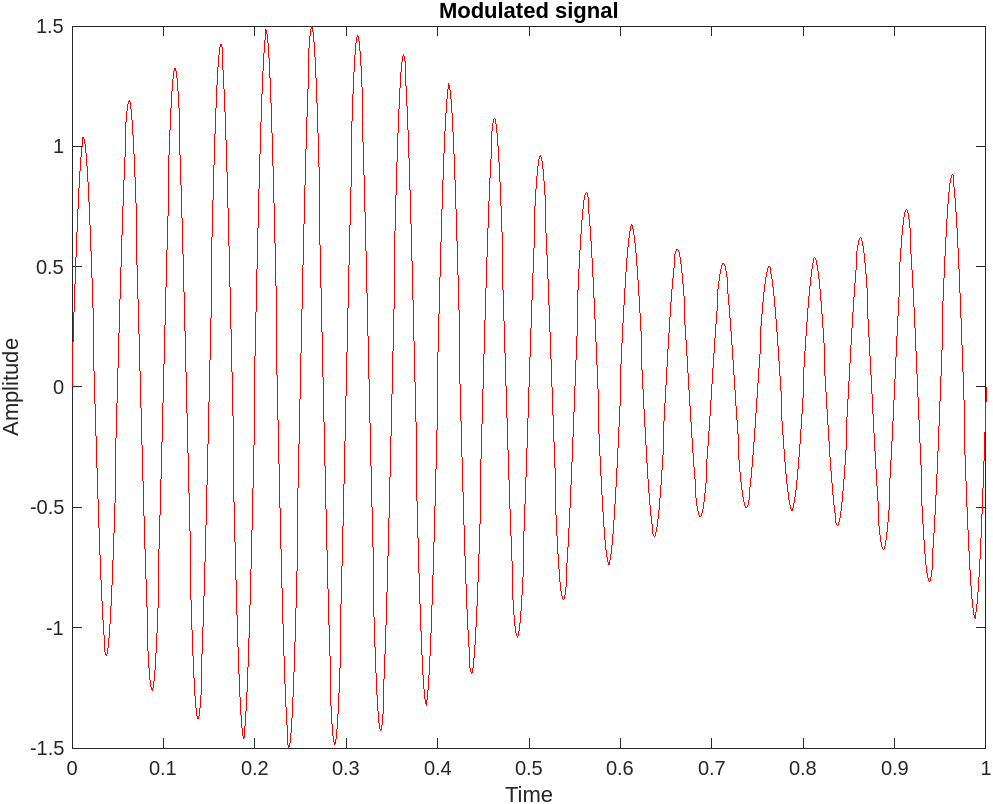
\includegraphics[width=\linewidth]{AMmudot5.png}
                \caption{\mu = 0.5}
                \label{img:AMmudot5}
            \end{subfigure}
            \begin{subfigure}{0.45\linewidth}
                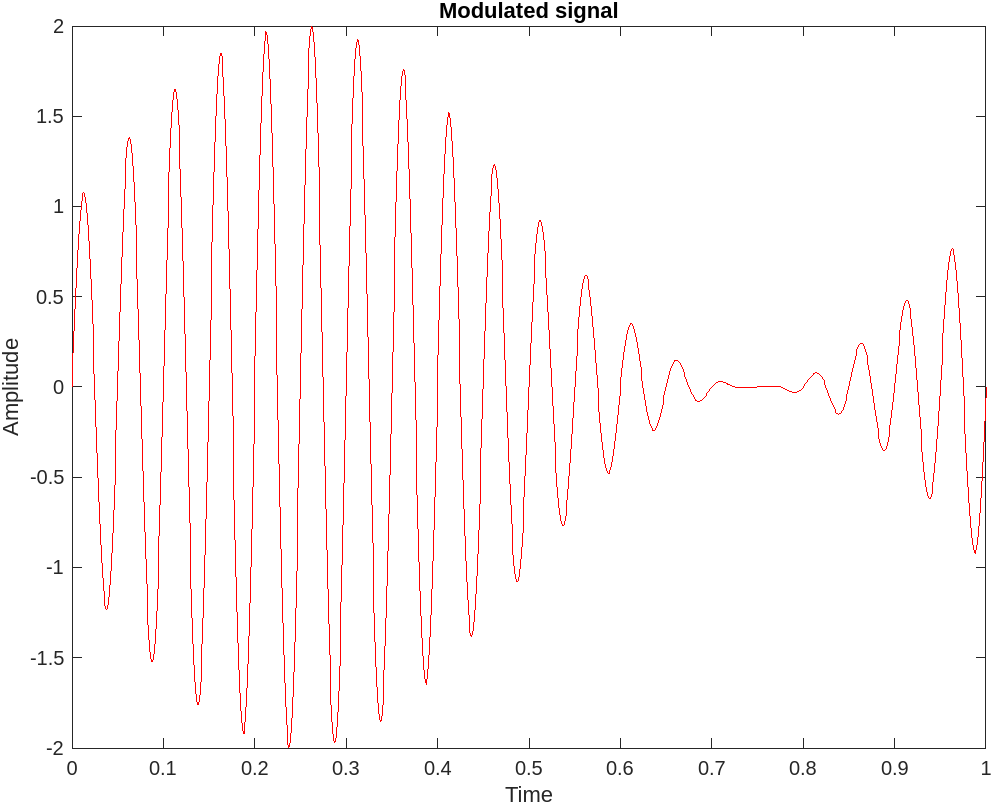
\includegraphics[width=\linewidth]{AMmu1.png}
                \caption{\mu = 1}
                \label{img:AMmu1}
            \end{subfigure}

            \caption{Σήμα Διαμορφωμένο κατά Πλάτος}
            \label{img:AMmu}
        \end{figure}

        Όταν το διαμορφωμένο σήμα φτάνει στο δέκτη, έχει τη μορφή:
        \begin{equation}
            \label{eq:AMrec}
            r(t) = \hat{A}\left[1+\mu \frac{m(t)}{m_p}\right]\cos(2\pi f_ct + \theta) + n(t)
        \end{equation}

        όπου το πλάτος του φέροντος $\hat{A}$ είναι συνήθως το πολύ μικρότερο από το πλάτος A του φέροντος
        που μεταδόθηκε, η γωνία \bm{\theta} αντιπροσωπεύει τη διαφορά φάσης μεταξύ των ταλαντωτών φορέα πομπού
        και δέκτη και \bm{n(t)} αντιπροσωπεύει τον θόρυβο. Θα ακολουθήσουμε μια κοινή πρακτική και θα
        αντισταθμίσουμε τη συχνότητα ταλαντωτή του δέκτη από τη φέρουσα συχνότητα $f_c$ του πομπού.
        Αυτό δίνει το σήμα:
        \begin{equation}
            \label{eq:AMfreqcomp}
            \hat{r}(t) = \hat{A}\left[1 + \mu \frac{m(t)}{m_p}\right]\cos(2\pi f_{IF}t + \theta) + n(t)
        \end{equation}
        όπου η λεγόμενη \textbf{ενδιάμεση συχνότητα} δίνεται από: \bm{$f_{IF} = f_c - f_o$}.
        Στο δέκτη, το σήμα \bm{$\hat{r}(t)$} μπορεί να περάσει μέσα από ένα φίλτρο διέλευσης ζώνης για να
        αφαιρεθούν οι παρεμβολές από ανεπιθύμητα σήματα σε συχνότητες κοντά στην \bm{$f_c$}. 
        Συνήθως το σήμα \bm{$\hat{r}(t)$} ενισχύεται επίσης. Η αποδιαμόρφωση του σήματος \bm{$\hat{r}(t)$}
        μπορεί να γίνει είτε με τη χρήση φωρατή περιβάλλουσας (envelope detector) είτε με τη χρήση 
        σύγχρονου ανιχνευτή AM. Ένας φωρατής περιβάλλουσας μπορεί να υλοποιηθεί ως ανορθωτής 
        ακολουθούμενος από ένα φίλτρο χαμηλής διέλευσης. Η περιβάλλουσα \bm{E(t)} του \bm{$\hat{r}(t)$}
        δίνεται από:
        \begin{equation}
            \label{eq:envelope}
            E(t) = \hat{A}\left[1 + \mu \frac{m(t)}{m_p}\right] = \hat{A} + \frac{\hat{A} \mu}{m_p}m(t)
        \end{equation}

    \section{\textbf{\textsf{Διαδικασία Εργαστηρίου}}}
        \subsection{\textsf{Προσομοίωση ΑΜ}}
            Αυτή η άσκηση σκοπεύει να προσομοιώσει ένα σήμα AM και να μελετήσει τις παραμέτρους του.
            \subsubsection*{\textsf{\underline{Πομπός ΑΜ}}}
            \begin{itemize}
                \item Ανοίξτε ένα καινούριο διάγραμμα ροής στο GNU Radio
                \item Ορίστε τις \textbf{Επιλογές Δημιουργίας} σε \textbf{QT GUI}.
                \item Ορίστε το \textbf{ρυθμό δειγματοληψίας} της \textbf{\textit{μεταβλητής}} σε \textbf{200k}.
                \item Προσθέστε ένα άλλο μπλοκ \textbf{\textit{μεταβλητής}},
                    ονομάστε το \textbf{freq} και ορίστε το σε \textbf{2k}.
                \item Προσθέστε ένα άλλο μπλοκ \textbf{\textit{μεταβλητής}}, 
                    ονομάστε το \textbf{TX\_freq} και ορίστε το σε \textbf{20k}.
                \item Προσθέστε μια \textbf{\textit{Πηγή Σήματος}} και ορίστε τον \textbf{Τύπο Εξόδου}
                σε \textbf{float}, την \textbf{Κυματομορφή} σε \textbf{συνημίτονο},\\
                την \textbf{Συχνότητα} σε \textbf{freq}, το \textbf{Πλάτος} σε \textbf{1} και τέλος 
                \textbf{\textit{Μετατόπιση}} σε \textbf{0}\footnote{
                    Ο ρυθμός δειγματοληψίας αναφέρεται επίσης στο ρυθμό με τον οποίο τα δείγματα
                    διέρχονται από το διάγραμμα ροής. Εάν δεν υπάρχει έλεγχος ρυθμού, ρολόι υλικού ή
                    μηχανισμός στραγγαλισμού, τα δείγματα θα παραχθούν, θα περάσουν από το διάγραμμα 
                    ροής και θα καταναλωθούν όσο το δυνατόν γρηγορότερα (δηλαδή το διάγραμμα ροής θα
                    είναι δεσμευμένο από την CPU). Μόνο ένα μπλοκ που αντιπροσωπεύει κάποιο υποκείμενο
                    υλικό με το δικό του ρολόι (π.χ. USRP, κάρτα ήχου) ή το throttle μπλοκ, θα
                    χρησιμοποιήσει το "Sample Rate" για να ρυθμίσει αυτό το ρολόι υλικού και επομένως 
                    θα έχει ως αποτέλεσμα την εφαρμογή ελέγχου ρυθμού στα δείγματα στο διάγραμμα ροής.
                }.
                \item Προσθέστε μια \textbf{\textit{Πολλαπλασιαστή Σταθερά}}, ορίστε τη \textbf{Σταθερά}
                    σε \textbf{0.5}. Αλλάξτε τον \textbf{Τύπο ΕισόδουΕξόδου} σε \textbf{float}.
                \item Προσθέστε μια \textbf{\textit{Σταθερή Πηγή}} και ορίστε τον \textbf{Τύπο Εξόδου}
                    σε \textbf{float} αριθμούς, ορίστε \textbf{Σταθερά} σε \textbf{1}.
                \item Προσθέστε ένα μπλοκ \textbf{\textit{Πρόσθεσης}}. Αλλάξτε τον \textbf{Τύπο ΕισόδουΕξόδου}
                 σε \textbf{float}. Συνδέσετε την \textbf{\textit{Σταθερή Πηγή}} και την
                 \textbf{\textit{Πολλαπλασιαστή Σταθερά}} στο μπλοκ \textbf{\textit{Πρόσθεσης}}.
                \item Προσθέστε ένα μπλοκ \textbf{\textit{Πολλαπλασιαστή}}, οριστε τον 
                 \textbf{Τύπο ΕισόδουΕξόδου} σε \textbf{float}.
                \item Προσθέστε μια \textbf{\textit{Πηγή Σήματος}}, ορίστε τον \textbf{Τύπο Εξόδου} σε
                 \textbf{float}, την \textbf{Κυματομορφή} σε \textbf{Συνημίτονο}, την \textbf{Συχνότητα} σε
                 \textbf{Tx\_freq}, το \textbf{Πλάτος} σε \textbf{1} και τέλος \textbf{Μετατόπιση} σε \textbf{0}.
                \item Προσθέστε ένα \textbf{\textit{QT GUI Sink}} και ορίστε τον \textbf{Τύπο} σε
                 \textbf{float} και το \textbf{FFT Size} σε \textbf{2,048 kHz}.
            \end{itemize}

            Τα παραπάνω μπλοκ κατασκευάζουν έναν πομπό AM εφαρμόζοντας την \ref{eq:AM}.
            Παρατηρήστε την κυματομορφή στο πεδίο χρόνου και συχνότητας.
            Κάθε μπλοκ στο GNURadio έχει μια \textbf{ενότητα σχολίων}. Για να το βρείτε, κοιτάξτε την καρτέλα
            για \textbf{Προχωρημένους} ενός μπλοκ. Προσδιορίστε τη λειτουργικότητα κάθε μπλοκ 
            στο σχέδιο τοποθετώντας μια μικρή σημείωση. Αυτή η σημείωση θα είναι ορατή στο διάγραμμα ροής.

            \subsubsection*{\textsf{\underline{Δέκτης ΑΜ}}}
            \begin{itemize}
                \item Χρησιμοποιήστε το διάγραμμα ροής πομπού AM.
                \item Προσθέστε ένα άλλο μπλοκ \textbf{\textit{μεταβλητής}}, 
                    ονομάστε το \textbf{Rx\_freq} και ορίστε το σε \textbf{15k}.
                \item Προσθέστε μια \textbf{\textit{Πηγή Σήματος}} και ορίστε τον \textbf{Τύπο Εξόδου}
                σε \textbf{float}, την \textbf{Κυματομορφή} σε \textbf{Συνημίτονο},\\
                τη \textbf{Συχνότητα} σε \textbf{Rx\_freq}, το \textbf{Πλάτος} σε \textbf{1} και τέλος 
                \textbf{Μετατόπιση} σε \textbf{0}.
                \item Προσθέστε ένα μπλοκ \textbf{\textit{Πολλαπλασιαστή}}, οριστε τον 
                 \textbf{Τύπο ΕισόδουΕξόδου} σε \textbf{float}.
                \item Προσθέστε ένα \textbf{\textit{Χαμηλοπερατό Φίλτρο}}, ορίστε το 
                 \textbf{Είδος Πεπερασμένης Κρουστικής Απόκρισης} σε \textbf{float}, 
                 την \textbf{Συχνότητα Αποκοπής} σε \textbf{10k} και το \textbf{Πλάτος μετάδοσης} σε \textbf{1k}.
                \item Προσθέστε ένα μπλοκ \textbf{\textit{Απόλυτης Τιμής}}. 
                 Ορίστε τον \textbf{Τύπο ΕισόδουΕξόδου} σε \textbf{float}.
                \item Προσθέστε ένα \textbf{\textit{Χαμηλοπερατό Φίλτρο}}, ορίστε το 
                 \textbf{Είδος Πεπερασμένης Κρουστικής Απόκρισης} σε \textbf{float}, 
                 την \textbf{Συχνότητα Αποκοπής} σε \textbf{2k} και το \textbf{Πλάτος μετάδοσης} σε \textbf{1k}.
                \item Προσθέστε ένα \textbf{\textit{QT GUI Sink}} και ορίστε το \textbf{Type} σε
                 \textbf{float}, και το \textbf{FFT Size} σε \textbf{2,048 kHz}.
            \end{itemize}
            Στο τέλος θα πρέπει να έχετε ένα διάγραμμα ροής όπως φαίνεται στο σχήμα(2). 
            Εκτελείτε το διάγραμμα ροής και λάβετε την έξοδο χρόνου και συχνότητας στα σημεία 
            A, B, C, D, E και F όπως φαίνεται στο σχήμα \ref{img:timefreq}. Αλλάξτε τον δείκτη διαμόρφωσης
            σε 0.25, 0.75 και 1. Ποια είναι η διαφορά στην κυματομορφή σήματος AM;
            \begin{figure}[h]
                \centering
                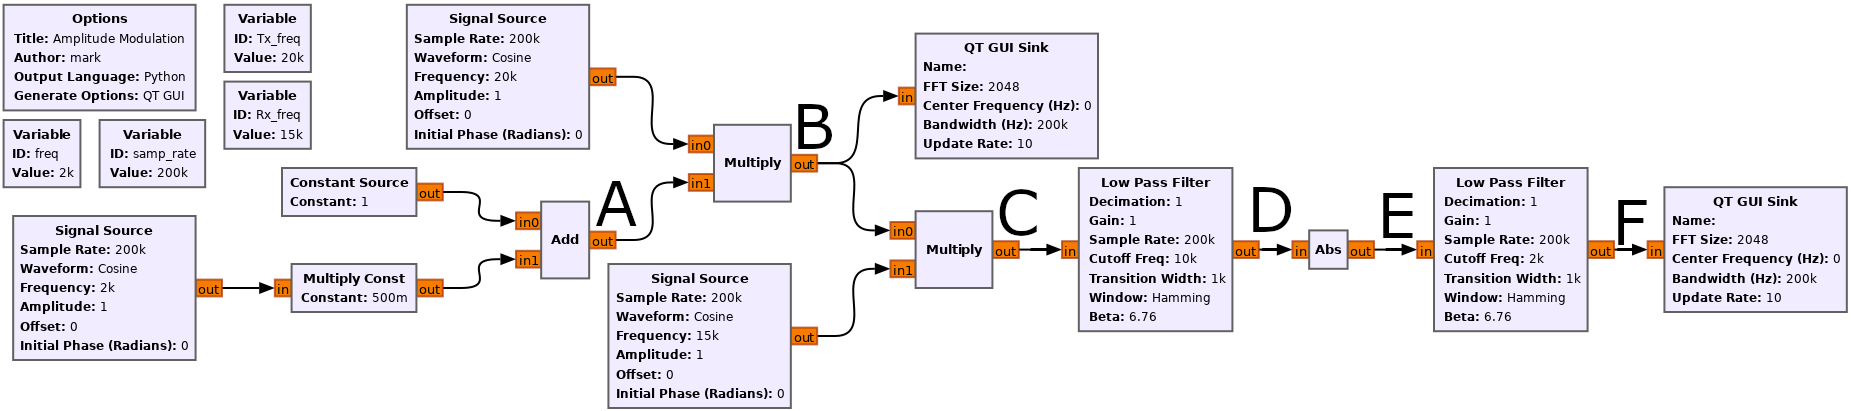
\includegraphics[width=\textwidth]{ex1Flow.png}
                \caption{Διαμόρφωση Πλάτους στο GNURadio}
                \label{img:ex1Flow}
            \end{figure}

            \begin{figure}[h]
                \centering
                \begin{tabular}{cccc}
                    \multicolumn{2}{c}{A} & \multicolumn{2}{c}{D} \\
                    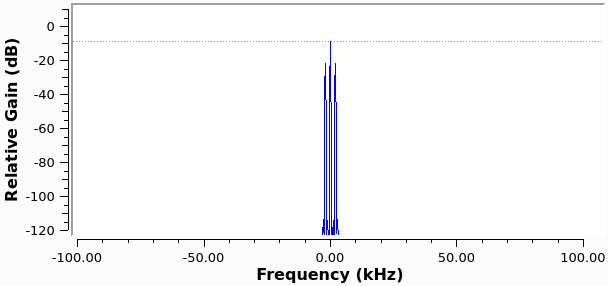
\includegraphics[width=.23\linewidth]{ex1Af.png} & 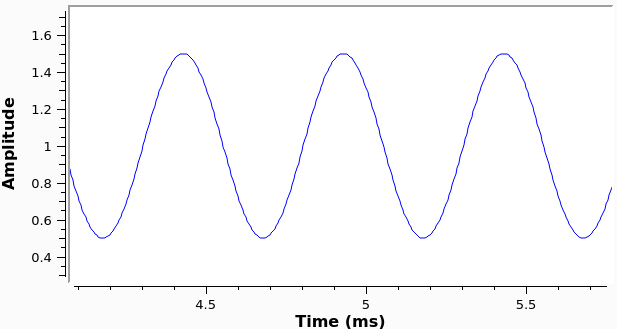
\includegraphics[width=.23\linewidth]{ex1At.png} & 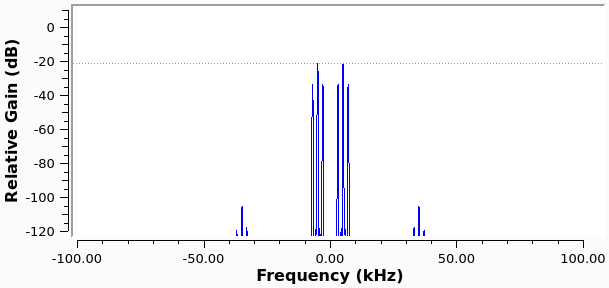
\includegraphics[width=.23\linewidth]{ex1Df.png} & 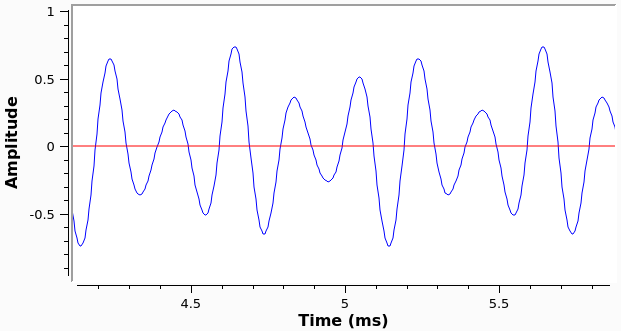
\includegraphics[width=.23\linewidth]{ex1Dt.png}\\
                    \multicolumn{2}{c}{B} & \multicolumn{2}{c}{E} \\
                    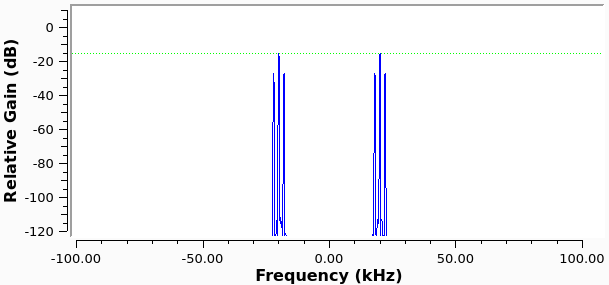
\includegraphics[width=.23\linewidth]{ex1Bf.png} & 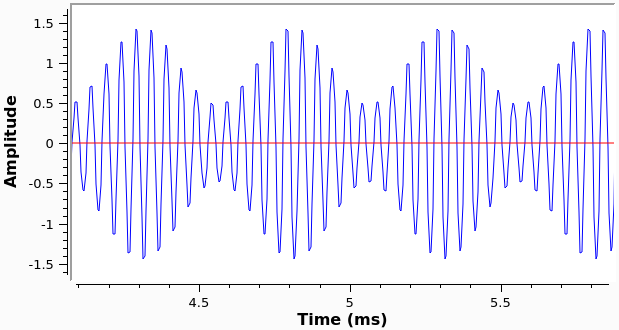
\includegraphics[width=.23\linewidth]{ex1Bt.png} & 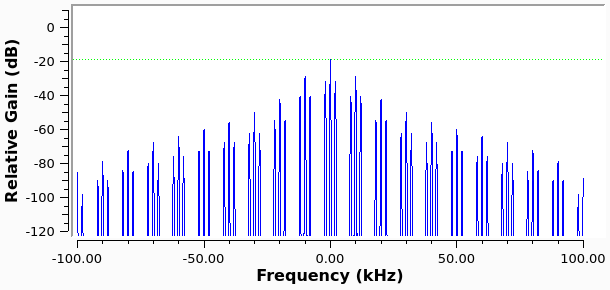
\includegraphics[width=.23\linewidth]{ex1Ef.png} & 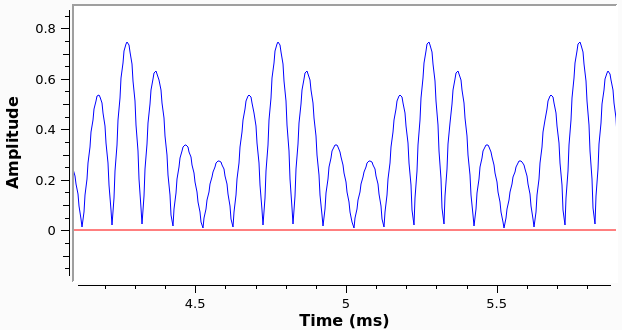
\includegraphics[width=.23\linewidth]{ex1Et.png}\\
                    \multicolumn{2}{c}{C} & \multicolumn{2}{c}{F}\\
                    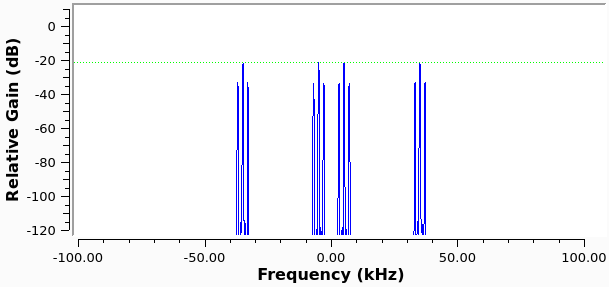
\includegraphics[width=.23\linewidth]{ex1Cf.png} & 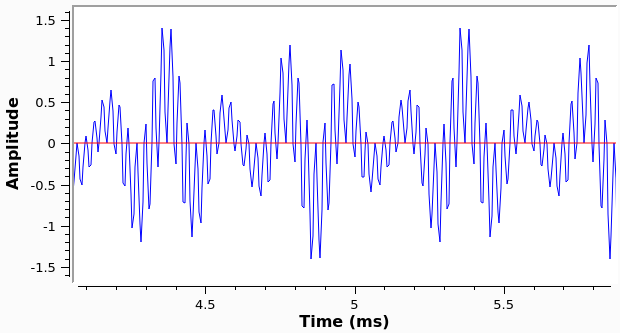
\includegraphics[width=.23\linewidth]{ex1Ct.png} & 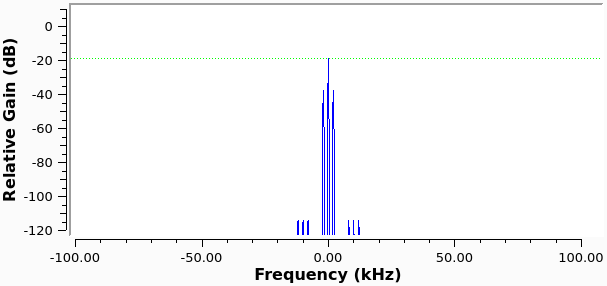
\includegraphics[width=.23\linewidth]{ex1Ff.png} & 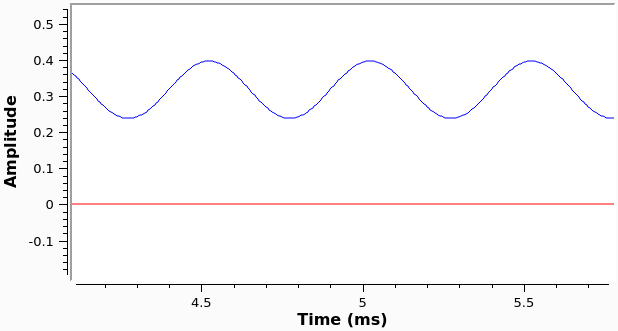
\includegraphics[width=.23\linewidth]{ex1Ft.png}
                \end{tabular}
                \caption{Τα πεδία χρόνου και συχνότητας για κάθε σημείο του γραφήματος (\ref{img:ex1Flow})}
                \label{img:timefreq}
            \end{figure}
            

    
    
\end{document}